\chapter{Data Understanding per Classi}
\label{ch:visual}

In questo capitolo si andranno a impiegare i due data set minimali, ottenuti mediante una massiccia aggregazione dei dati a disposizione effettuata nella precedente fase di \textit{preprocessing}, come base per l'utilizzo di alcune tecniche di visualizzazione. \\

Il fine è quello di evidenziare elementi che facciano intuire un \textit{trend} fra le varie \textbf{classi di record} in cui si è aggregato tutti i dati a disposizione: si sta parlando, ovviamente, delle \textit{coorti di immatricolazione} per quanto riguarda il data set degli studenti, e degli \textit{Anni Accademici} riguardo alle valutazioni dei corsi.

\section{Valutazione dei Corsi}

Per la valutazione dei corsi, si lavorerà sul dataset ottenuto come descritto nella Sezione \ref{prepr:eval_min}. Data la sua dimensione molto ristretta, è possibile riportarlo qui sotto per intero:

\begin{table}[]
\begin{tabular}{lllll}
\hline
A.A. & Val. Media & Std. Dev. Media & \% Val. Suff. & N. Val. \\ \hline
2010-2011 & 7.54 & 1.74 & 82.14 & 17 \\
2011-2012 & 7.93 & 1.61 & 90.68 & 26 \\
2012-2013 & 7.98 & 1.7 & 90.55 & 30 \\
2013-2014 & 7.7 & 1.77 & 87.17 & 47 \\
2014-2015 & 7.94 & 1.77 & 89.36 & 51 \\
2015-2016 & 8.01 & 1.76 & 89.94 & 49 \\
2016-2017 & 8.01 & 1.82 & 89.34 & 53 \\ \hline
\end{tabular}
\end{table}

    \subsection{Panoramica Generale sulle Valutazioni dei Corsi}
    \label{visual:eval_gen}

    Per inquadrare subito la situazione e mettere a fuoco con un singolo colpo d'occhio le caratteristiche di ogni Anno Accademico, è stato realizzato l'istogramma mostrato in Figura \ref{eval_gen}. \\

    Come si può facilmente verificare con una rapida osservazione del grafico, l'unico attributo che varia sensibilmente è il numero medio di valutazioni dei corsi registrate; si può notare inoltre che esso presenta una tendenza a crescere con l'avanzare dell'Anno Accademico. Per quanto riguarda gli altri attributi, rimangono sostanzialmente simili, fatta eccezione per la percentuale di valutazioni sufficienti registrata negli Anni Accademici 2010-2011, leggermente inferiori rispetto agli altri. \\

    \begin{figure}
        \centering
        \caption{istogramma mostrante una panoramica generale su tutti gli attributi del dataset descritto in Sezione \ref{prepr:eval_min}}
        \label{eval_gen}
        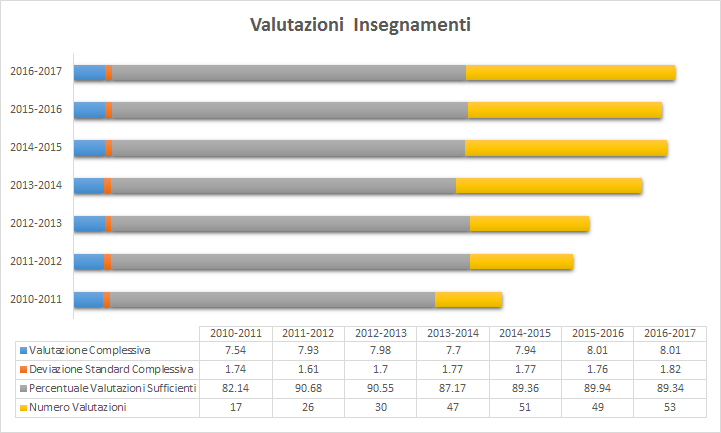
\includegraphics[scale=0.55]{../visual/eval_3.png}
    \end{figure}

    \subsection{Dettaglio sulla Percentuale di Valutazioni Sufficienti}

    Volendo vedere con un maggior livello di dettaglio l'andamento di quest'ultimo aspetto, è stato realizzato un grafico mostrante le percentuali di valutazioni dei corsi sufficienti come serie storica attraverso tutti gli Anni Accademici per i quali si hanno a disposizione delle informazioni. Tale grafico, mostrato in Figura \ref{eval_p}, mostra con maggiore chiarezza quanto si è osservato sull'istogramma generale di Figura \ref{eval_gen}. \\

    \begin{figure}
        \centering
        \caption{serie storica dell'attributo "percentuale di valutazioni sufficienti" attraverso gli Anni Accademici coperti dal data set delle valutazioni dei corsi}
        \label{eval_p}
        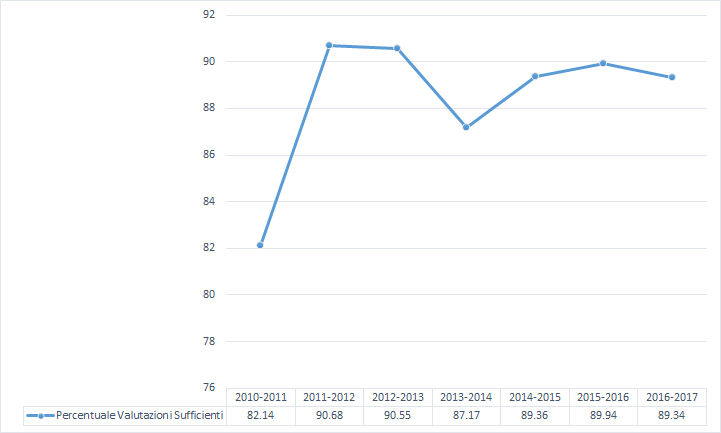
\includegraphics[scale=0.56]{../visual/eval_2.png}
    \end{figure}

\section{Produttività degli Studenti}

    Riguardo ai dati relativi alla produttività degli studenti, il dataset su cui si è lavorato è quello descritto nella Sezione \ref{prepr:stud_min}. Esso è già stato riportato nella sua interezza in tale sede ma, data la sua piccola dimensione, è comunque ripetuto qui di seguito per comodità di consultazione. \\

    \begin{tabular}{llllll}
		\hline
		Coorte & N. & Laureati {[}\%{]} & Test Ingresso & Voto & Ritardo \\ \hline
		2010 & 30 & 6.67 & 15.4 & 25.5 & 0.81 \\
		2011 & 39 & 10.26 & 13.26 & 24.81 & 1.07 \\
		2012 & 58 & 25.86 & 14.05 & 24.79 & 1.01 \\
		2013 & 80 & 11.25 & 14.39 & 24.98 & 0.77 \\ \hline
	\end{tabular}

    \subsection{Panoramica generale sulla Produttività degli Studenti}

    Per quanto riguarda una preliminare analisi generale dell'intero data set, restano valide le considerazioni espresse in Sezione \ref{visual:eval_gen}. Pertanto, è stato generato un istogramma del tutto analogo a quanto fatto tale Sezione, mostrato in Figura \ref{stud_gen}. \\

    In seguito a una analisi visiva del grafico, si può notare come gli attributi che più variano sono il numero di studenti imatricolati e la percentuale di studenti laureati entro la fine del periodo in esame. L'andamento degli studenti immatricolati è considerevolmente simile a quello riscontrato sul numero di valutazioni dei corsi registrate, quindi è plausibile supporre una certa correlazione diretta fra i due attributi --- piuttosto banalmente, se ci sono più studenti iscritti, perverranno anche più valutazioni dei corsi.

    \begin{figure}
        \centering
        \caption{istogramma mostrante una panoramica generale su tutti gli attributi generali del dataset descritto in Sezione \ref{prepr:stud_min}}
        \label{stud_gen}
        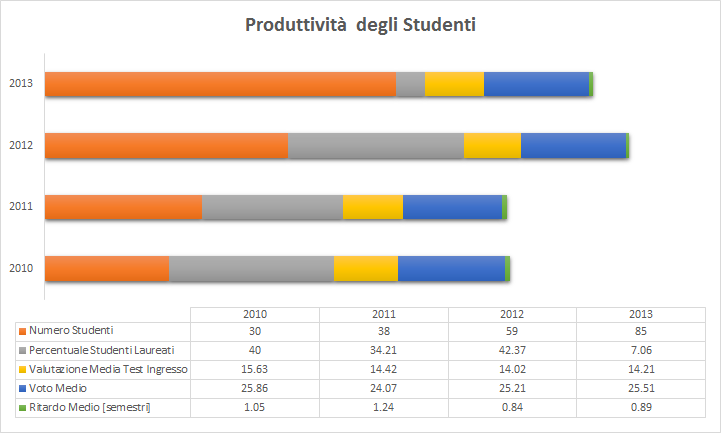
\includegraphics[scale=0.50]{../visual/stud_1.png}
    \end{figure}

    \subsection{Relazione fra Test di Ingresso, Voto Medio e Ritardo}

    Un aspetto curioso sul quale si è voluto fare luce è l'esistenza o meno di una qualche correlazione fra il risutlato conseguito nel test di ingresso e le valutazioni ottenute nei successivi esami di profitto. Avendo a disposizione in questa sede entrambi gli attributi in forma aggregata, è stato realizzato il grafico di Figura \ref{test}. \\

    Si noti che gli attributi considerati non esprimono valori nella stessa scala: il test di ingresso prevede un punteggio massimo di 25, mentre per gli esami di profitto il punteggio massimo previsto è di 31 punti\footnote{I voti negli esami vanno ovviamente da 18 a 30, con il 31 a rappresentare in realtà il 30 con lode.}. C'è stato perciò bisogno di effettuare una \textit{normalizzazione} di tali attributi, per poterli confrontare direttamente. \\

    \begin{figure}
        \centering
        \caption{serie temporale mostrante i valori degli attributi normalizzati "voto medio" e "valutazione media al test di ingresso"}
        \label{test}
        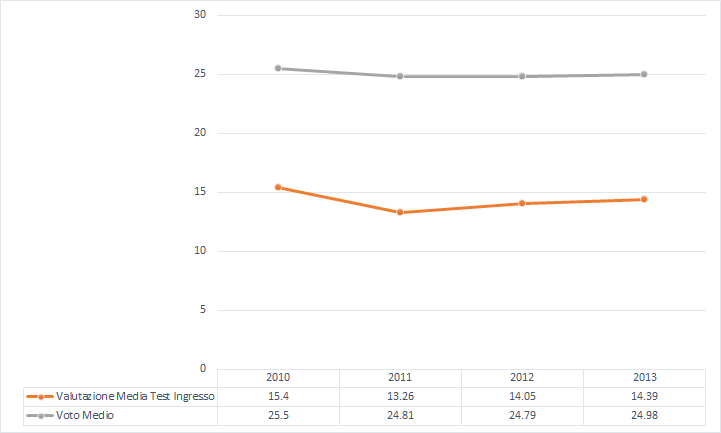
\includegraphics[scale=0.55]{../visual/stud_2.png}
    \end{figure}

    Come si può vedere, pare esserci una correlazione estremamente blanda, ma non risulta così significativa da essere presa in considerazione per ulteriori approfondimenti. Inoltre, si può notare un \textit{offset} abbastanza pronunciato fra i due attributi; concedendoci una speculazione, potrebbe essere dato da un minor impegno degli studenti nel test di ingresso dato dalla sua soglia di sufficienza molto bassa --- 12 punti su 25 --- e dal fatto che il risultato in tale test non impatta in alcun modo la futura carriera accademica. \\

    \begin{figure}
        \centering
        \caption{serie temporale mostrante l'andamento dell'attributo "ritardo medio" relativo al superamento degli esami di profitto}
        \label{ritardo}
        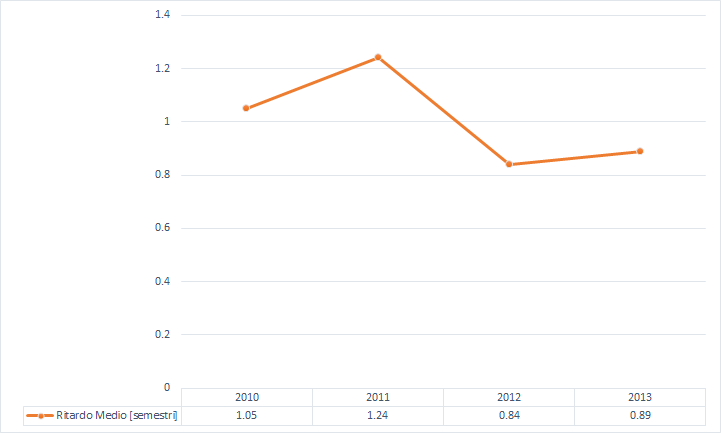
\includegraphics[scale=0.55]{../visual/stud_3.png}
    \end{figure}

    La curiosa flessione della valutazione al test di ingresso fra la coorte di studenti immatricolati nel 2011 trova un riscontro nell'andamento del ritardo medio con cui sono stati superati gli esami di profitto rispetto al loro primo appello, come si può vedere dalla Figura \ref{ritardo}. Comunque, si tratta di una correlazione abbastanza debole, pertanto è stato scelto di limitarsi a notarla, senza proseguire nell'analisi. \\

    \subsection{Percentuale di Studenti Laureati}

    Un indice interessante dell performances di una certa coorte di immatricolazione è la percentuale di studenti che ha terminato con successo il corso di studi entro il periodo di tre anni considerato dai dati a disposizione. Si è quindi deciso di porre attenzione su questo attributo, mostrandolo come serie temporale in Figura \ref{laureati}. \\

        \begin{figure}
        \centering
        \caption{serie temporale mostrante l'andamento dell'attributo "percentuale di studenti laureati entro tre Anni Accademici dall'immatricolazione"}
        \label{laureati}
        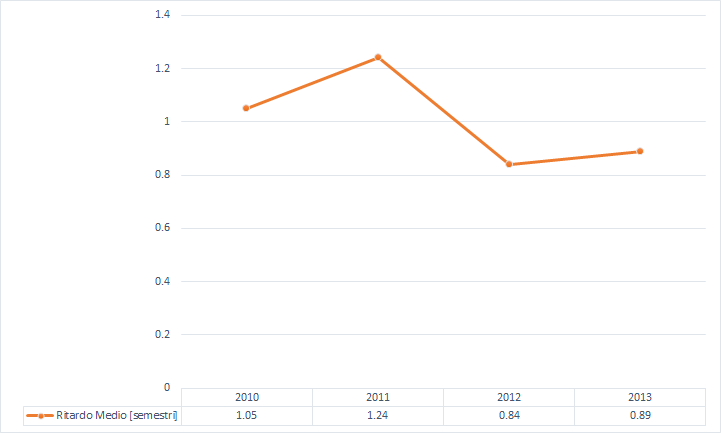
\includegraphics[scale=0.55]{../visual/stud_3.png}
    \end{figure}

    Si nota una sensibile oscillazione di questo valore, che tocca il suo picco massimo nella coorte di studenti immatricolati nel 2012, ma non si è riscontrato --- almeno in seguito a una preliminare analisi visiva --- alcuna correlazione con altri aspetti evidenziati da altri attributi.
